\documentclass[
  manuscript=article,  %% article (default), rescience, data, software, proceedings, poster
  layout=preprint,  %% preprint (for submission) or publish (for publisher only)
  year=20xx,
  volume=x,
]{extra/joas}

\doi{xx.xxxxx/joas.xxxx.xxxx}

% \conference{} command is only used for proceedings
\conference{Conference Title}

\received {1 April 20xx}
\revised  {1 May 20xx}
\accepted {10 May 20xx}
\published{20 May 20xx}

\editor{Editor Name}

\reviewers{First Reviewer, Second Reviewer, Third Reviewer}


% --- blew is the area for authors ---

% remove the following two packages, and delete all \blindtext commands
\usepackage[english]{babel} 
\usepackage{blindtext}
% Extra useful packages
\usepackage{xspace}
\usepackage{mathtools}

\usepackage{amsmath,amsfonts,amssymb}
%\usepackage{algorithmic}
%\usepackage{graphicx}
%\usepackage{textcomp}
\usepackage{xcolor}

% special circle character    
\def\invcircledast#1{%
  \mathbin{\vphantom{\circledast}\text{%
    \ooalign{\smash{\blackcircle}\cr
             \hidewidth\smash{\textcolor{white}{\bf \footnotesize $#1$}}\hidewidth\cr
            }%
  }}%
}
\newcommand{\blackcircle}{\raisebox{-.6ex}{\scalebox{2.30}{$\bullet$}}}

% Name
\newcommand{\Design}{$\mathsf{DiTTO}$\xspace}
\newcommand{\Designn}{PersonalizedHD\xspace}

% Math
%\usepackage{amsthm}
\newtheorem{prop}{Proposition}
\usepackage{multirow}

\usepackage{kotex}

% Space control
\renewcommand{\baselinestretch}{0.97}
\setlength{\textfloatsep}{1pt}
\setlength{\dbltextfloatsep}{1pt}

\newcommand{\todo}[1]{{\color{red}{#1}}}
\newcommand{\ys}[1]{{\color{blue}{#1}}}

\newcommand{\Figure}{Fig.}


% specify the .bib file for references
\addbibresource{reference.bib} 


% Make sure your article tile is within 12 words
\title{DiTTO : A Diffusion-Based Framework for Configurable and Realistic Storage Trace Generation}

\author{Seohyun Kim (202328003)}
\affiliation{M.S. Candidate | Artificial Intelligence, DGIST }
\email{selenium@dgist.ac.kr} 

% \author{Second Author \orcid{0000-0000-0000-0000}}
% \affiliation{Institution-2, City, Country}

% \author{Third Author}
% \alsoaffiliation{Institution-1, City, Country}
% \affiliation{Institution-3, City, Country}


% maximum five keywords
\keywords{benchmark; diffusion; generative model} 

% Important: don't over use abbreviations. Only use abbreviation if the term is used more than ten times throughout the paper. Otherwise, write them in full.


\begin{document}

\begin{abstract}
We propose \Design, a novel diffusion-based framework for generating realistic, precisely configurable, and diverse multi-device storage traces. Leveraging advanced diffusion techniques, \Design enables the synthesis of high-fidelity continuous traces that capture temporal dynamics and inter-device dependencies with user-defined configurations. Our experimental results demonstrate that \Design can generate traces with high fidelity and diversity while aligning closely with guided configurations with only 8\% errors.
\end{abstract}


\section{Introduction}


Understanding and optimizing the performance of distributed storage systems require detailed workload analysis in various environments such as RAID arrays and CephFS. Realistic workload traces, which capture read and write operations across multiple devices, are crucial for identifying performance bottlenecks and evaluating optimization strategies such as caching policies and load balancing. However, collecting real-world traces is costly and often impractical due to high instrumentation overheads and privacy concerns. This lack of accessible traces hinders the development of data-driven storage optimizations and limits the evaluation of emerging techniques.

To mitigate this, synthetic trace generation tools such as SPEC Storage allows for controlled workload simulation. While useful, these tools rely on predefined templates and fail to capture the complex, evolving behavior of real-world workloads. Machine learning-based methods~\cite{paul2022machine} attempt to improve realism but are still constrained by excessive feature engineering by human experts to identify application-specific characteristics.

In this paper, we propose \Design (\underline{\textbf{Di}}ffusion-based \underline{\textbf{T}}race generation and \underline{\textbf{T}}emporal \underline{\textbf{O}}utpainting), a \textit{diffusion-based} generative framework for producing realistic and configurable multi-device storage traces. Unlike conventional generative approaches that rely on predefined patterns or static sampling, our framework provides \textit{precise, user-controlled}, and \textit{arbitrary-length} trace generation, enabling workloads to be synthesized according to quantifiable constraints such as read/write ratios, access burstiness, and temporal dependencies.

\Design transforms raw access logs, including timestamps, operation types, and device identifiers, into structured\ multi-channel representations, enabling diffusion models to capture complex temporal dependencies and cross-device correlations. We introduce a workload conditioning mechanism that explicitly embeds quantifiable user-defined parameters into the generative process, providing fine-grained control over trace characteristics. Unlike conventional text-based conditioning in image diffusion models~\cite{dalle2}, our approach ensures explicit and constrained output control. Additionally, we design a sparsity-aware training approach to ensure that long periods of inactivity and bursty access patterns are accurately modeled. Finally, by leveraging outpainting techniques, a generative technique that extends content while preserving contextual coherence, \Design produces traces of arbitrary length while maintaining contextual consistency. In this paper, we make the following contributions.


\noindent 1) We propose a \textbf{diffusion-based synthetic trace generation framework} that accurately captures multi-device workload patterns through structured representations. To the best of our knowledge, it is the \underline{first work} that utilizes the diffusion technique for the storage trace generation. 

\noindent 2) We present a novel \textbf{quantifiable workload conditioning mechanism} that ensures quantifiable control over key workload properties such as read/write ratios.

\noindent 3) We design \textbf{sparsity-aware training} and \textbf{outpainting-based trace generation} techniques to generate workloads with long inactive periods and extended trace durations.

\noindent 4) We show that \Design can generate high-fidelity storage traces that replicate real-world workload characteristics while preserving trace diversity with less than 8\% error.

\begin{figure}
    \centering
    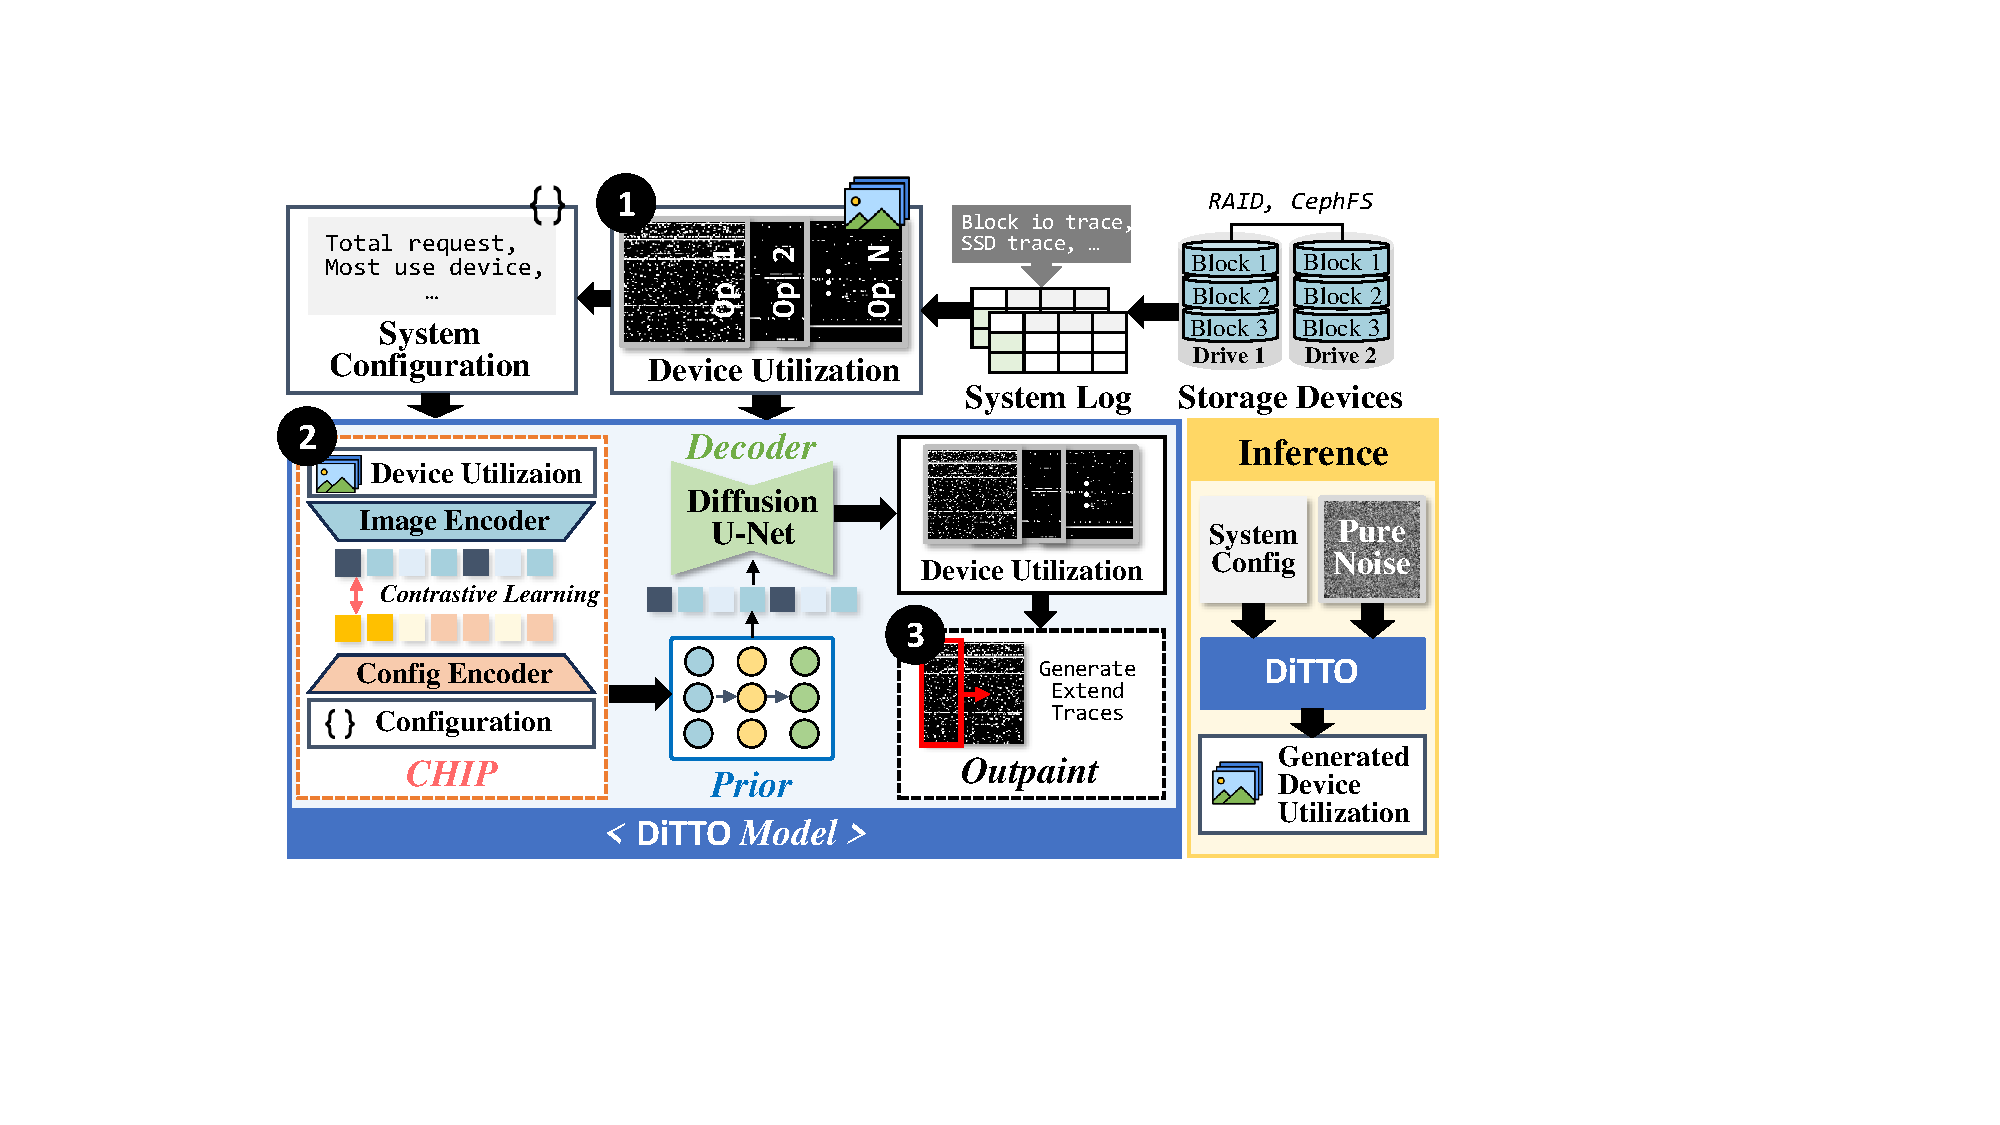
\includegraphics[width=0.9\columnwidth]{figure/overview.pdf}
    \caption{Overview of \Design}
    \label{fig:overview}
\end{figure}



\section{Proposed Technique: \Design}  
We propose \Design, a novel diffusion-based framework for generating realistic, configurable, and diverse multi-device storage traces. The framework captures intricate temporal dynamics and inter-device dependencies while allowing users to specify workload characteristics. The overall pipeline of \Design is illustrated in Fig.~\ref{fig:overview}, consisting of three main stages: $\invcircledast{1}$ transforming traces into structured image representations, $\invcircledast{2}$ encoding numeric workload characteristics for explicit conditioning, and $\invcircledast{3}$ generating arbitrarily long traces using a diffusion-based model enhanced with outpainting.

\noindent {\bf Transforming system traces into image-based representations.}  
\Design first converts raw per-device access logs into structured multi-channel image representations, enabling the diffusion model to learn workload patterns effectively. Each input trace consists of timestamped read and write operations mapped to corresponding storage devices. To construct the image representation, we segment time into fixed intervals along the x-axis, while the y-axis corresponds to different storage devices. Each pixel encodes the presence of a read or write event at a specific time interval and device, with separate channels distinguishing operation types.  
Storage workloads exhibit extreme sparsity, where access events are interspersed with long periods of inactivity. To mitigate this, we introduce local Gaussian noise augmentation, which creates smooth intensity gradients around access events. This prevents excessive sparsity in the image representation, improving the diffusion model to learn contextual relationships across time and devices.  

\noindent {\bf Encoding numeric workload characteristics.}  
A key requirement for synthetic trace generation is the ability to precisely control workload properties including read/write ratios, request rates, and device utilization patterns. To achieve this, we introduce CHIP (Contrastive Hyperconfiguration-Image Pretraining), a novel embedding mechanism that conditions the model on user-defined workload parameters.  
CHIP operates by mapping \textit{numeric workload configurations} into a latent space that aligns with the image-based representations of system traces. This is achieved via contrastive learning~\cite{clip}, where the model learns to associate similar workload characteristics with similar trace representations. Given a workload configuration, CHIP generates an embedding that guides the diffusion process, ensuring that generated traces adhere to the specified workload properties. Unlike conventional text-based conditioning in image diffusion models, CHIP explicitly enforces \textit{quantifiable constraints}, making it well-suited for structured data synthesis.  

\noindent {\bf Generating continuous traces.}  
Since real-world storage workloads span arbitrary durations, \Design must generate long sequences while preserving workload characteristics. To achieve this, we incorporate outpainting, a generative technique that extends trace durations while maintaining contextual coherence.  
The outpainting works by conditioning the diffusion model on the final states of previously generated traces, allowing seamless extension over time. Specifically, when generating a new trace segment, the model samples latent variables from the boundary of the prior output, ensuring that patterns such as periodic bursts, coordinated device accesses, and workload fluctuations remain consistent. This prevents abrupt transitions and maintains statistical fidelity across extended traces.  


\ifx{
\section{Proposed Technique: \Design}
In this paper, we present \Design, a novel diffusion-based framework for generating realistic, configurable, and diverse multi-device storage traces. The framework captures the intricate temporal dynamics and inter-device dependencies characteristic of real-world workloads while supporting user-defined configurations for tailored trace generation. By leveraging a diffusion-based modeling approach inspired by DALL·E 2\cite{dalle2}, \Design synthesizes high-fidelity storage traces as structured data representations, meeting the requirements of diverse evaluation scenarios.


The training begins with transforming raw per-device access logs collected on a multi-storage environment into image representations, where each channel in the image corresponds to the operation type (read or write) and includes which storage devices are accessed within a fixed time window. This structured format enables the model to capture temporal patterns and inter-device correlations. User-defined configurations, including read/write ratios, device utilization patterns, and total requests, are embedded through our proposed embedding model, called CHIP (Contrastive Hyperconfiguration-Image Pretraining), which converts these annotations to the image-based workload representations in an embedding space. The CHIP embedding conditions the diffusion process via a prior, ensuring that generated traces reflect specified configurations. A UNet-based decoder then generates synthetic images from the latent representations, producing snapshots of system traces for fixed durations. For longer time horizons, \Design employs an outpainting technique to extend traces while maintaining temporal consistency.

\noindent {\bf Transforming system traces into image-based representations} Storage traces are characterized by infrequent events interspersed with long periods of inactivity, making direct encoding ineffective for generative modeling. To address this, \Design augments the image-like representation by introducing Gaussian noise around each access point. In this representation, the x-axis corresponds to time intervals within a fixed window, and each row along the y-axis is associated with a specific storage device. Each access event is encoded as a white pixel within the respective channel. 
Gaussian noise is applied locally around pixels to create a smooth intensity gradient, mitigating sparsity and enhancing the diffusion model's ability to capture contextual patterns around access events while maintaining spatial coherence.
% To mitigate the sparsity, Gaussian noise is applied locally around the pixel, creating a smooth intensity gradient. This augmentation not only reduces sparsity but also ensures that the diffusion model captures contextual patterns around access events while preserving spatial coherence in the image. (서현 수정)

\noindent {\bf Encoding numeric workload characteristics} To control the trace generation with fine-grained conditioning, e.g., read/write ratios or total requests, we devise the CHIP model, which maps numeric configurations into embedding vectors compatible with the image-based trace representations. CHIP aligns the high-dimensional numeric inputs with the latent space of the diffusion model using a contrastive learning approach. This alignment ensures that user-defined configurations, including quantifiable parameters like workload intensity or device utilization patterns, are accurately encoded as conditioning inputs.
%These embeddings guide the diffusion process, enabling \Design to generate traces that reflect specific workload characteristics with high fidelity.

\noindent {\bf Generating continuous trace} To extend generated traces beyond a fixed time window, \Design employes an outpainting technique that sequentially extends the trace while maintaining temporal and spatial consistency. Outpainting involves generating new trace segments by conditioning the model on the boundary of the previously generated trace. This approach preserves the contextual relationships across time intervals and ensures that patterns such as periodic bursts or coordinated device access are carried forward seamlessly. 
}\fi

\section{Experimental Results}

\begin{figure}
    \centering
    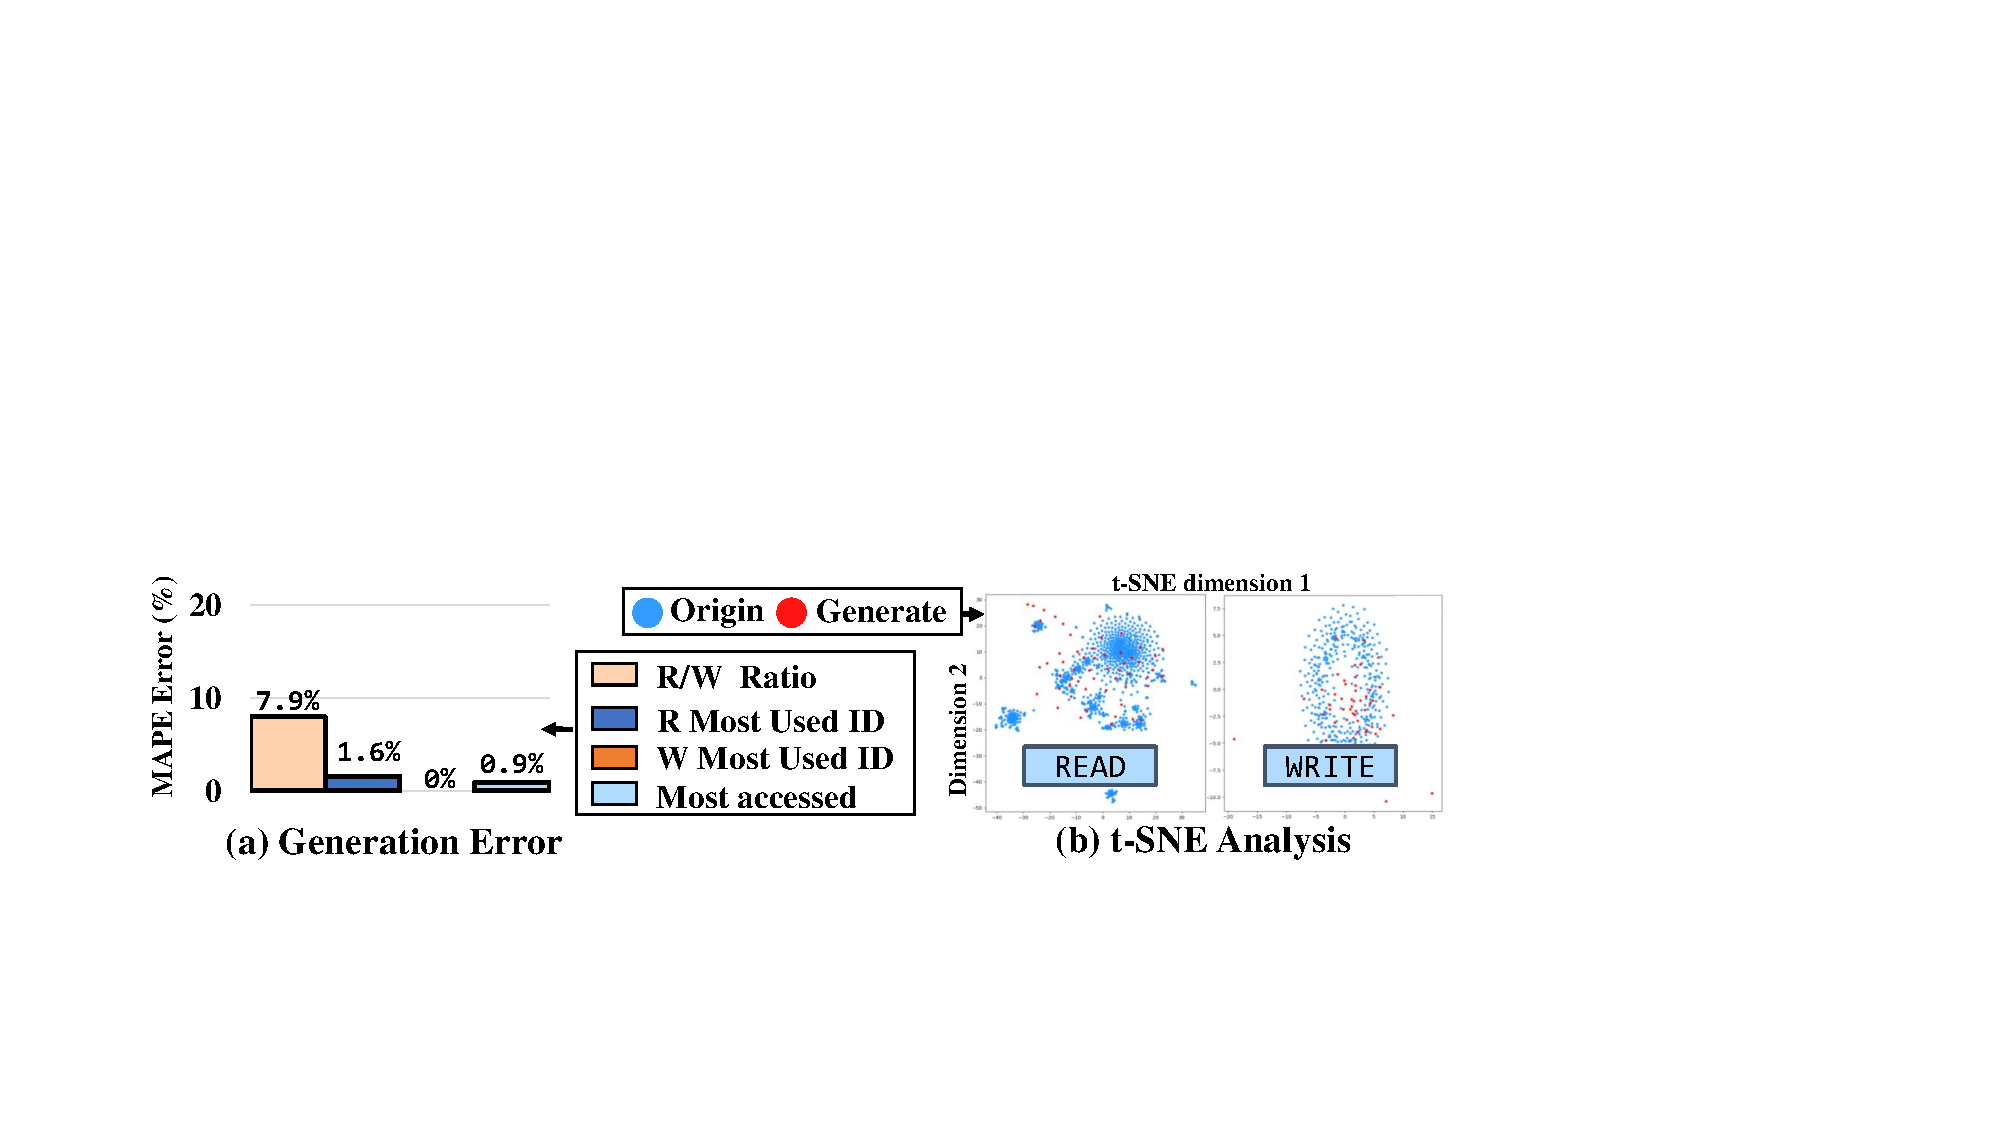
\includegraphics[width=0.9\columnwidth]{figure/eval.pdf}
    \caption{Generation error and t-SNE}
    \label{fig:eval}
\end{figure}


\begin{figure}
    \centering
    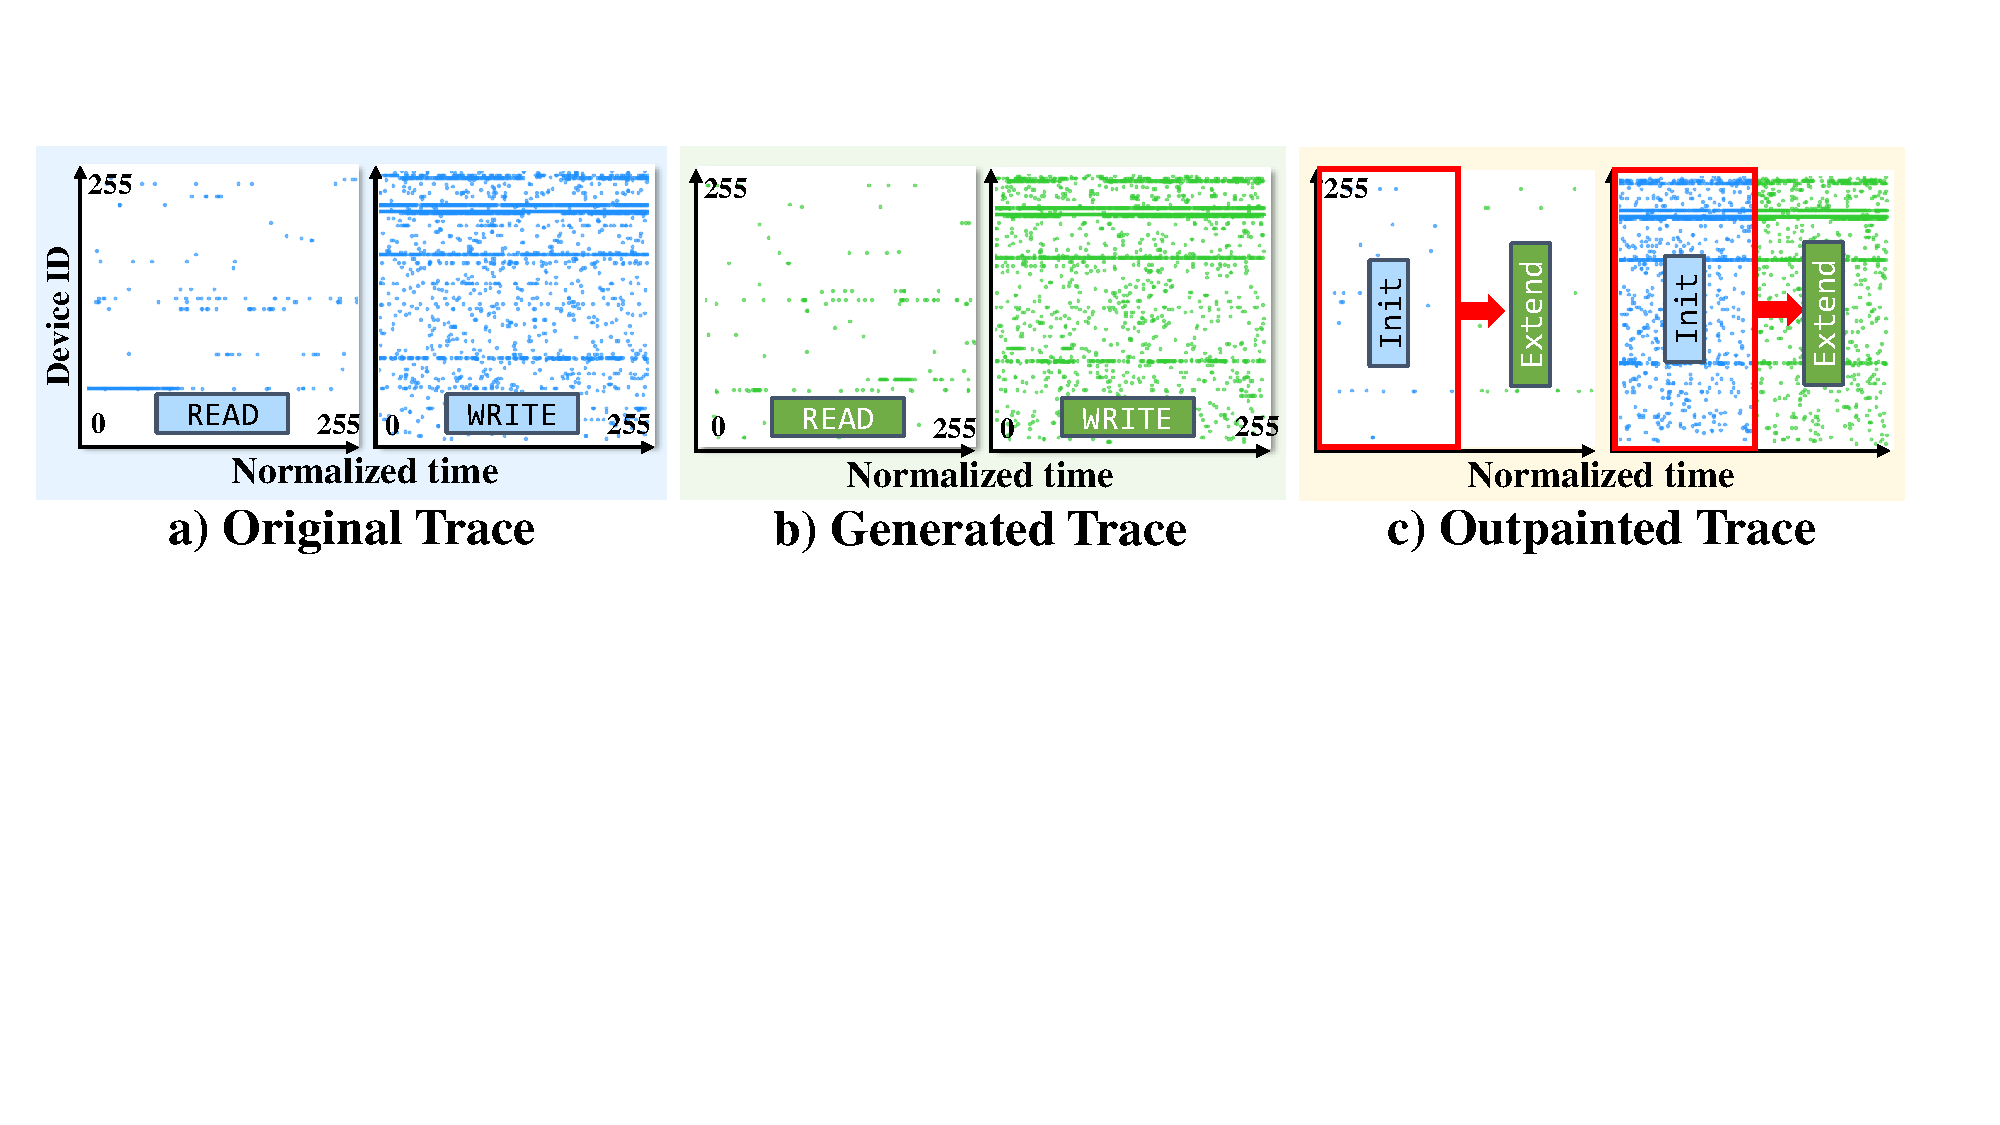
\includegraphics[width=0.9\columnwidth]{figure/result.pdf}
    \caption{(a), (b) Comparison between the original and generated traces, (c) Extended trace with collected data and configuration (Outpainting)}
    \label{fig:img}
\end{figure}

\begin{figure}
    \centering
    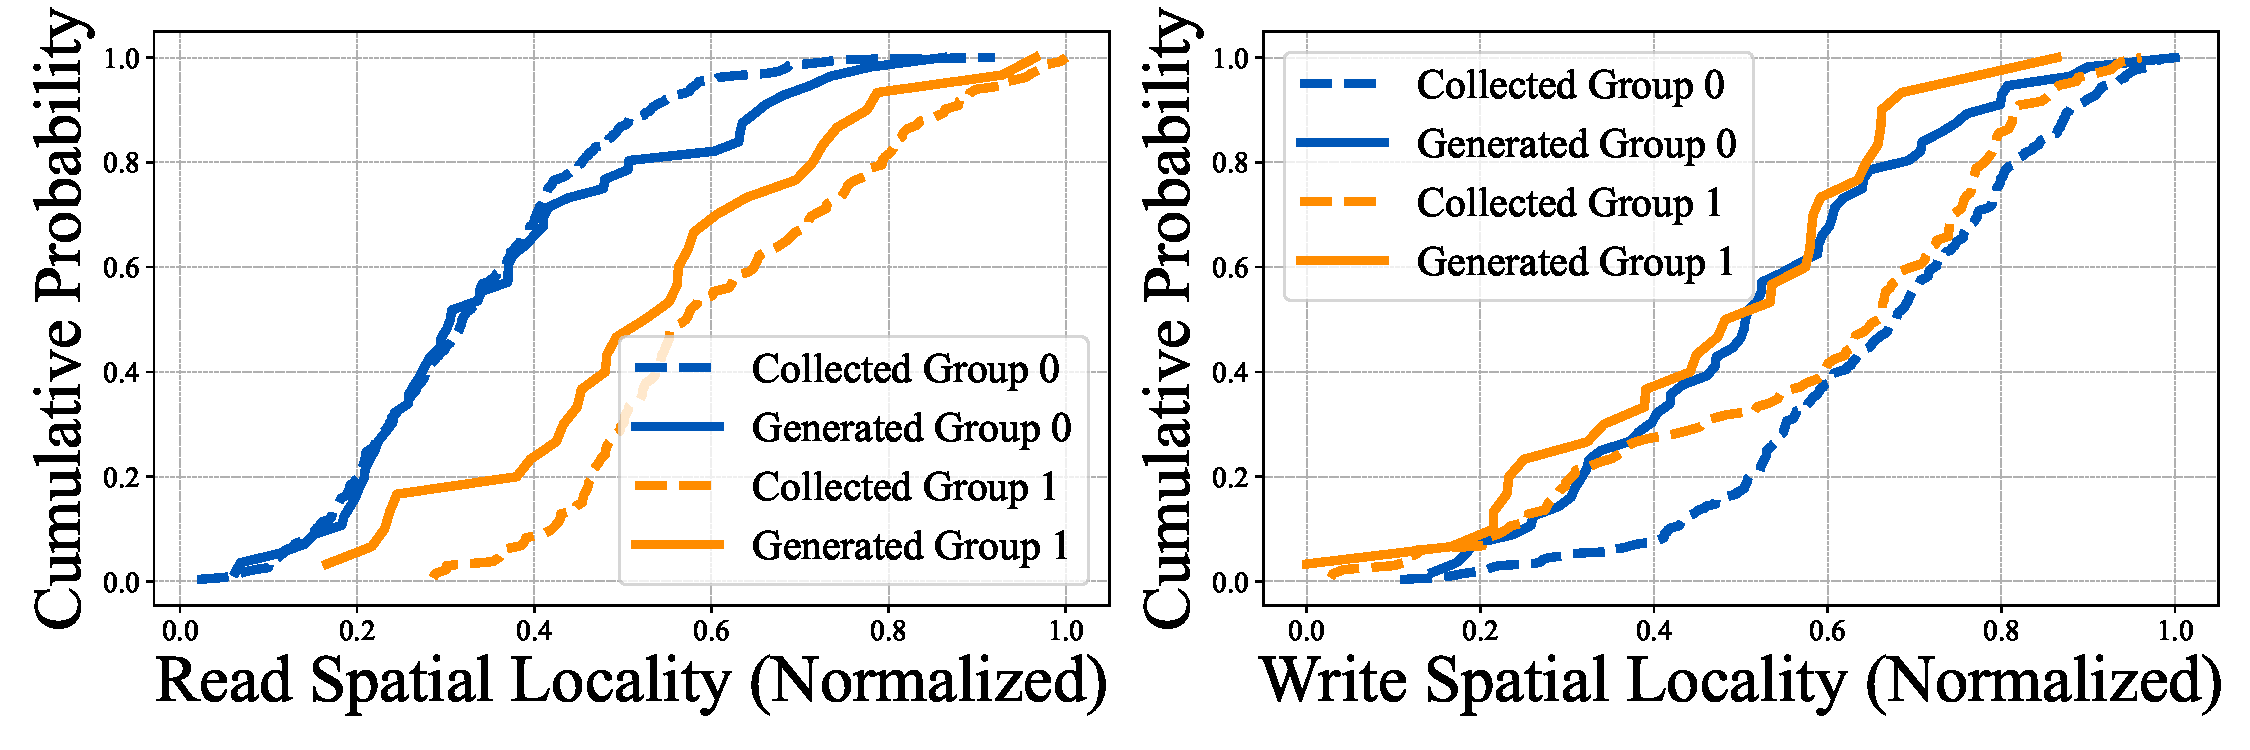
\includegraphics[width=0.9\columnwidth]{figure/locality.pdf}
    \caption{Distribution of spatial locality for different configuration groups}
    \label{fig:distribution}
\end{figure}

%\noindent {\bf Experimental Setup.} 
We implemented \Design using Pytorch 2.4 and evaluated the efficacy using Alibaba Block IO trace dataset.
%All experiments were performed on a machine equipped with an NVIDIA A100 GPU.
One of the key features of \Design is its ability to generate realistic traces that closely adhere to user-specified configurations, such as read/write ratios and workload intensity. Figure~\ref{fig:eval}(a) presents the evaluation results for 50 generated traces, reporting the errors in how well the traces follow the user configurations. The results show that \Design achieves an average error of less than 8\% for read/write ratios and 2\% for device utilization patterns, demonstrating its precision in capturing workload characteristics. Additionally, the t-SNE analysis in Figure~\ref{fig:eval}(b) indicates that the generated traces exhibit trends similar to real (\textsf{Origin}) traces while maintaining sufficient diversity. These results confirm that the CHIP model effectively embeds quantifiable characteristics into the trace generation process. For instance, when tasked with generating traces for a read-heavy workload (82.99\% reads), \Design produces traces with a read ratio of 81.24\%, closely aligning with the intended configuration.  

Figure~\ref{fig:img} compares synthetic traces to their real-world counterparts to illustrate the fidelity of \Design. The results show that the generated traces (b) closely resemble real-world traces (a) under the same workload configuration, capturing realistic access patterns. Figure~\ref{fig:img}(c) demonstrates the results of the outpainting technique. The results present that \Design extends traces over a longer time horizon while preserving the consistency of previously observed patterns.

To further demonstrate how \Design generates distinguishable traces under different conditions, we clustered the collected traces into two groups and then generated traces by sampling the corresponding configurations of each cluster. Figure~\ref{fig:distribution} presents the distribution of real and generated traces in terms of read/write spatial locality. The results indicate that \Design successfully generates distinct traces that align with the patterns observed in each cluster, despite spatial locality \textit{not being explicitly included} in the user-configurable parameters. This suggests that \Design not only follows explicit workload parameters but also learns and preserves \textit{underlying high-level workload characteristics}, such as spatial locality, by capturing underlying access patterns from real traces.  

\section{Conclusion}
We propose \Design, which generates synthetic traces for distributed storage systems by introducing a diffusion-based framework. By integrating sparsity-aware training, CHIP for fine-grained conditioning, and outpainting for extended durations, \Design effectively captures intricate temporal and spatial patterns of real workloads. Our evaluation shows that \Design can generate realistic traces aligned with user configurations with the error of less than 8\%.



\section{Future Plans}
Our current research is focused on fully developing the Image to Trace conversion process. Moving forward, we plan to refine this process to ensure the generated traces can be seamlessly reverted and evaluated within benchmark simulators. Additionally, we aim to develop a user-friendly framework that integrates the entire process, from trace generation to performance evaluation.


\printbibliography


\end{document}